\textbf{Name:} Patrick L. Harvey\\

\medskip

\textbf{Conspirators:}\\
McCarthy, Cormac\\
Gallagher, Ryan. J.\\
Morgan R. Frank\\
Lewis Mitchell\\
Aaron J. Schwartz\\
Andrew J. Reagan\\
Christopher M. Danforth\\
and Peter Sheridan Dodds\\
\textit{Generalized Word Shift Graphs:}\\
\textit{A Method for Visualizing and Explaining Pairwise Comparisons Between Texts.}\\
EPJ Data Science 10, no. 4 (2021).

\medskip
\medskip

\hrule

\medskip


\assignmentsonly{Goal: A paper per text studied, building through assignments.}

\begin{enumerate}

\item (3 points each)

  Using your text of choice, generate word shifts comparing two ``interesting'' regions of text.

  Use the Python package described in Ref.[\href{https://arxiv.org/abs/2008.02250}{1}].

  (Various Matlab versions made by the Unreliable Deliverator do exist and need to be shared on Gitplaces.)

  Links to paper versions (arXiv is always best),
  Github repository,
  and an
  exhilarating Twitter feed
  can be found here: \url{https://pdodds.w3.uvm.edu/research/papers/gallagher2021a/}.

  ``Interesting'' is anything you find interesting.  Could be books 3 and 12 in a series,
  second half of a book compared to the first half, season 4 of a show versus all seasons, etc.

  Aim to find two texts that are both reasonably large (more than $10^{4}$ words)
  and fairly different in average happiness scores (though even the same scores can be
  meaningfully explored with word shifts).
  
  Let's call the two texts
  $\texta$
  and
  $\textb$.
  In your plots, you should label them meaningfully based on your choices).

  Use a reasonable exclusion lens of your choice, e.g., [4, 6] or [3, 7].

  \begin{enumerate} 
  \item 
    Produce a word shift comparing text $\textb$ relative to text $\texta$.
    Use the average happiness of text $\texta$ as the baseline.
  \item 
    Interpret the word shift. Does what you see make sense?
    Are there any surprises?
    Are some words being used in what the average person might not think is their primary meaning?
    For example, ``crying'' in Moby Dick means yelling, and ``sick'' can mean ``awesome.''
  \item
    Produce a word shift comparing text $\texta$ relative to text $\textb$.
    Use the average happiness of text $\textb$ as the baseline.
  \item
    Comment on any asymmetries you see (the basic word shifts we use are asymmetric).
  \item
    Produce a word shift comparing text $\texta$ relative to text $\textb$.
    Now use 5 as the baseline reference score (neutral on the happiness-sadness spectrum of 1--9).
  \item
    Compared to your first word shift, how interpretable is this one?
  \end{enumerate}
\clearpage
  
   \solutionstart
  % Using your text of choice, generate word shifts comparing two ``interesting'' regions of text.

  % Use the Python package described in Ref.~\cite{gallagher2021a}.

  % (Various Matlab versions made by the Unreliable Deliverator do exist and need to be shared on Gitplaces.)

  % Links to paper versions (arXiv is always best),
  % Github repository,
  % and an
  % exhilarating Twitter feed
  % can be found here: \url{https://pdodds.w3.uvm.edu/research/papers/gallagher2021a/}.

  % ``Interesting'' is anything you find interesting.  Could be books 3 and 12 in a series,
  % second half of a book compared to the first half, season 4 of a show versus all seasons, etc.

  % Aim to find two texts that are both reasonably large (more than $10^{4}$ words)
  % and fairly different in average happiness scores (though even the same scores can be
  % meaningfully explored with word shifts).
  
  % Let's call the two texts
  % $\texta$
  % and
  % $\textb$.
  % In your plots, you should label them meaningfully based on your choices).

  % Use a reasonable exclusion lens of your choice, e.g., [4, 6] or [3, 7].
   
  \begin{enumerate}[wide, labelwidth=!, labelindent=0pt]
  \item
    % Produce a word shift comparing text $\textb$ relative to text $\texta$.
    % Use the average happiness of text $\texta$ as the baseline.
    
    The figure below compares Cormac McCarthy's \textit{Blood Meridian} (1985) with \textit{The Road} (2006).
    For the remainder of this assignment,
    \textit{Blood Meridian} will be referred to as $\texta$; \textit{The Road} will be $\textb$.

    The sub-figure on the left compares the weighted average shift of lexical happiness from $\texta \to \textb$;
    the right figure displaying the entropy shift with respect to lexical happiness from $\texta \to \textb$. For this assignment, we will not examine the entropy shifts, however they are included for reference.
    
    The lensing interval used here is $[4,6]$, 
    using a reference value equal to the average happiness of lensed $\texta (5.243)$.

    \begin{center}
        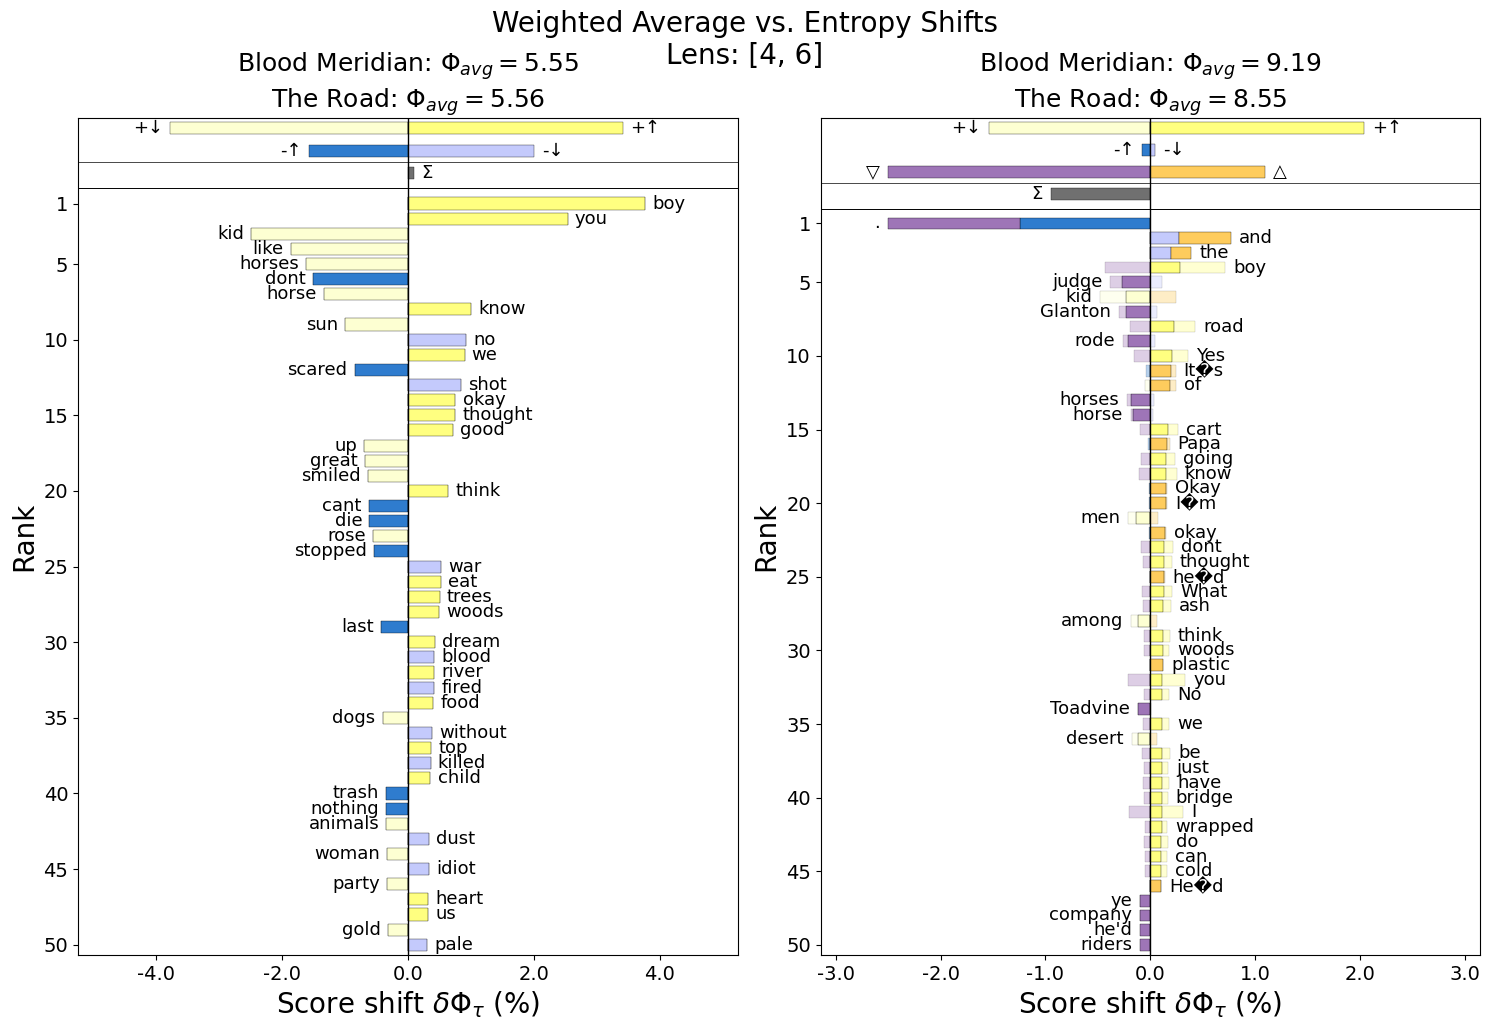
\includegraphics[width=\linewidth]{figures/21_1_a.png}
    \end{center}
    \clearpage
    
    The lensing interval used here is $[3,7]$, 
    using a reference value equal to the average happiness of lensed $\texta (5.266)$

    \begin{center}
        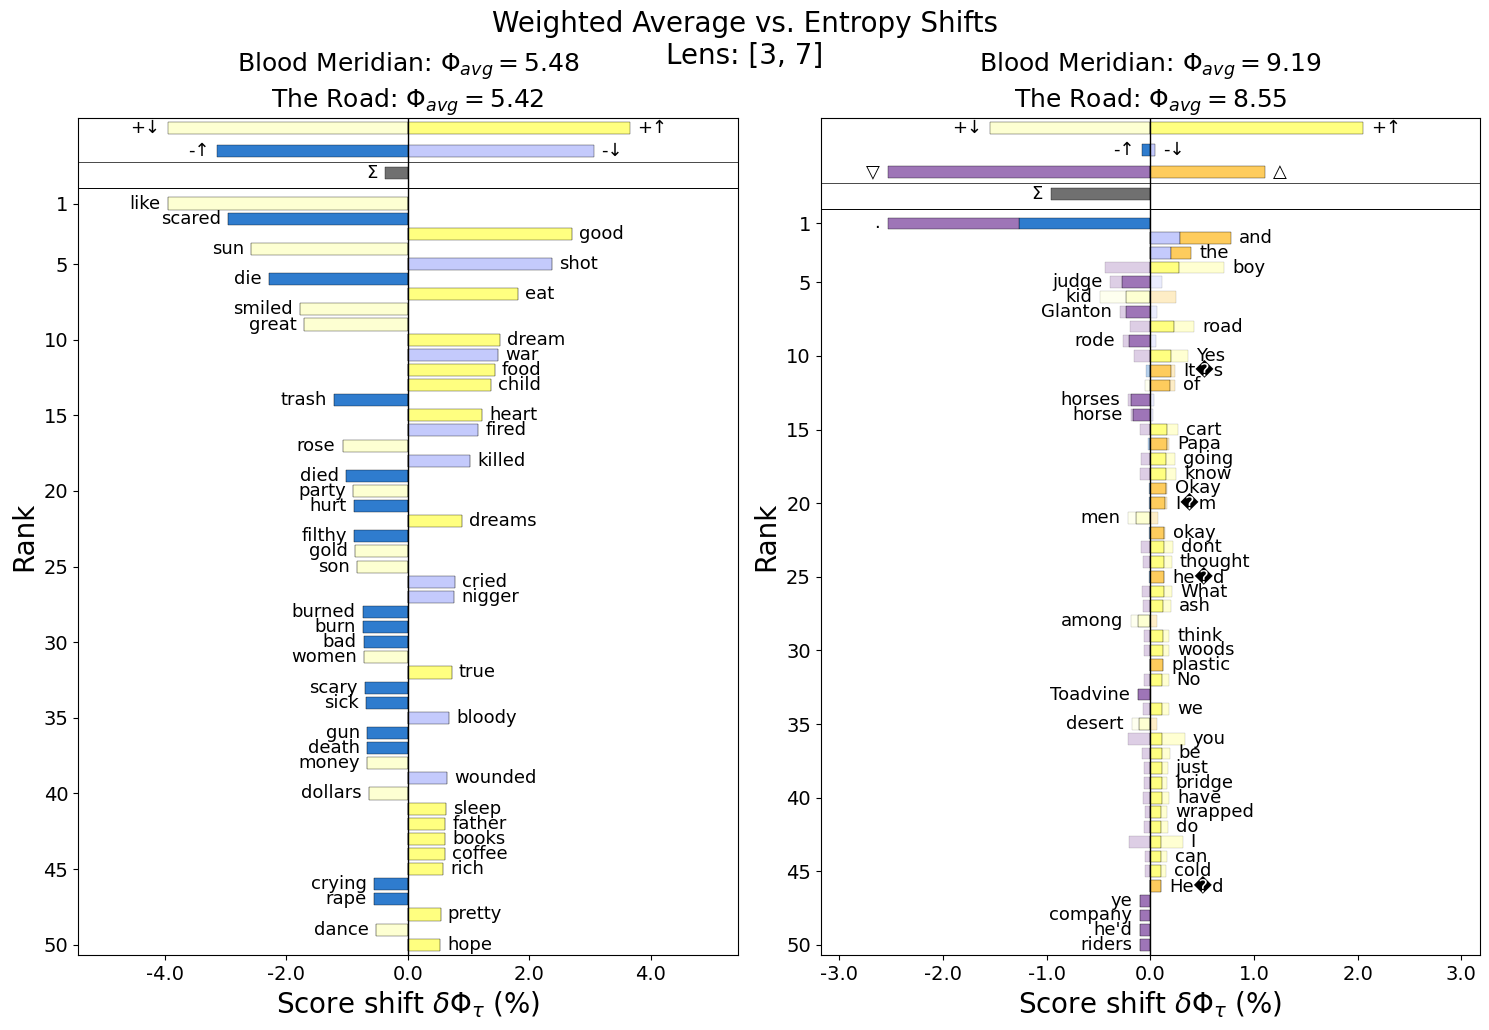
\includegraphics[width=\linewidth]{figures/21_1_a2.png}
    \end{center}

  \item 
    % Interpret the word shift. Does what you see make sense?
    % Are there any surprises?
    % Are some words being used in what the average person might not think is their primary meaning?
    % For example, ``crying'' in Moby Dick means yelling, and ``sick'' can mean ``awesome.''
    The results here make sense with respect to McCarthy's diction.
    It is important to note, however, that words which may generally have a "happy" connotation do not in the context of these works.

    For example, "party", "gold", "money", "dollars", and "dance" are often used in the context of a party of bandits, dancing over a slain person, or the seizing of material objects.

    The sentiment assigned to "like" is inappropriate in terms of McCarthy's diction, as it is often used to portray a simile. It would be nice if there were things in the novel which were objectively likeable, however it is like you are looking through a window where native peoples are beheaded for dollars. Needless to say, there is not much like the unflinching violence portrayed in $\texta$

    The only surprise, for me at least, is that $\texta$ is more gruesome than I remembered. While $\textb$ does not spare any details with respect to the brutality of life, there is a sense of hope portrayed by the author which is made evident in these comparisons.

    We see how narrowing the lens from $\pm 2$ to $\pm 1$
    
  \item
    % Produce a word shift comparing text $\texta$ relative to text $\textb$.
    % Use the average happiness of text $\textb$ as the baseline.
    Sticking with a reference value of $[3, 7]$ and using happiness average of $\textb (\Phi_{avg} = 5.280)$, but swapping the positions of $\texta$ and $\textb$ we have the figure below:

    \begin{center}
        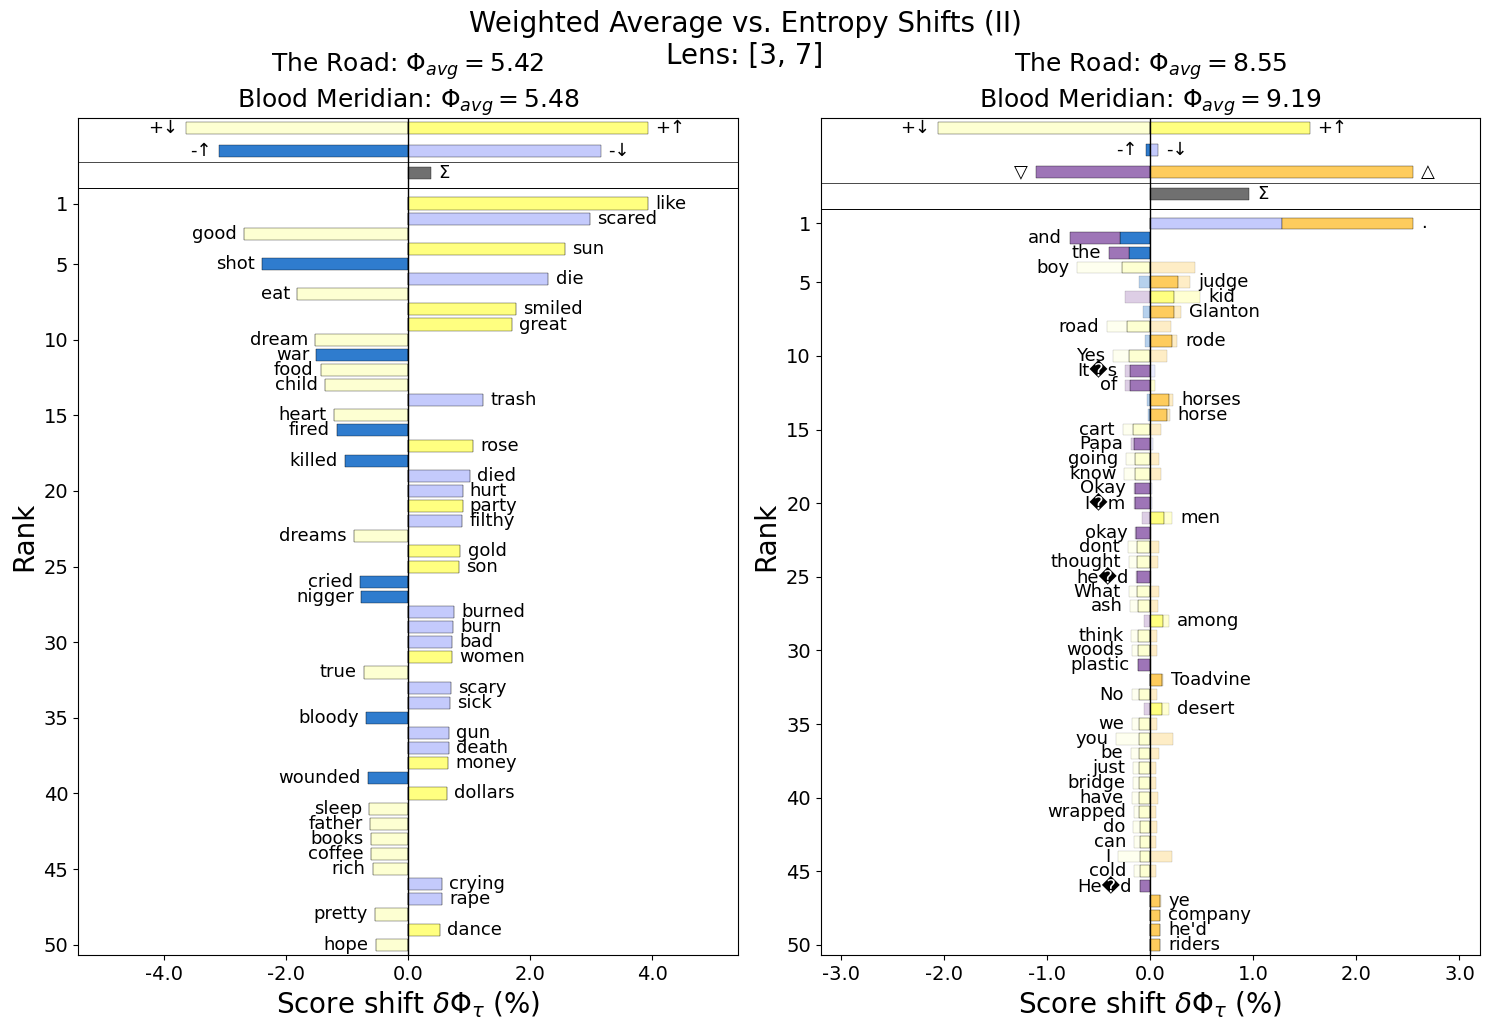
\includegraphics[width=\linewidth]{figures/21_1_c.png}
    \end{center}
    
  \item
    % Comment on any asymmetries you see (the basic word shifts we use are asymmetric).
    Let's start with the less than happy words identified for each.

    $\texta$ has 15 of the 23 negative words within the top 50 contributing words for weighted average shift.

    The scale of the frequency distributions with respect to their contributions towards the weighted average shift is greater in the $\texta$ direction (see $\Sigma$).
    \clearpage
    
  \item
    % Produce a word shift comparing text $\texta$ relative to text $\textb$.
    % Now use 5 as the baseline reference score (neutral on the happiness-sadness spectrum of 1--9).
    The top figure uses a reference value of 5, while the bottom figure is the first real figure, re-presented as a reference for the rhetor's relief from readjustment.
    
    \begin{center}
        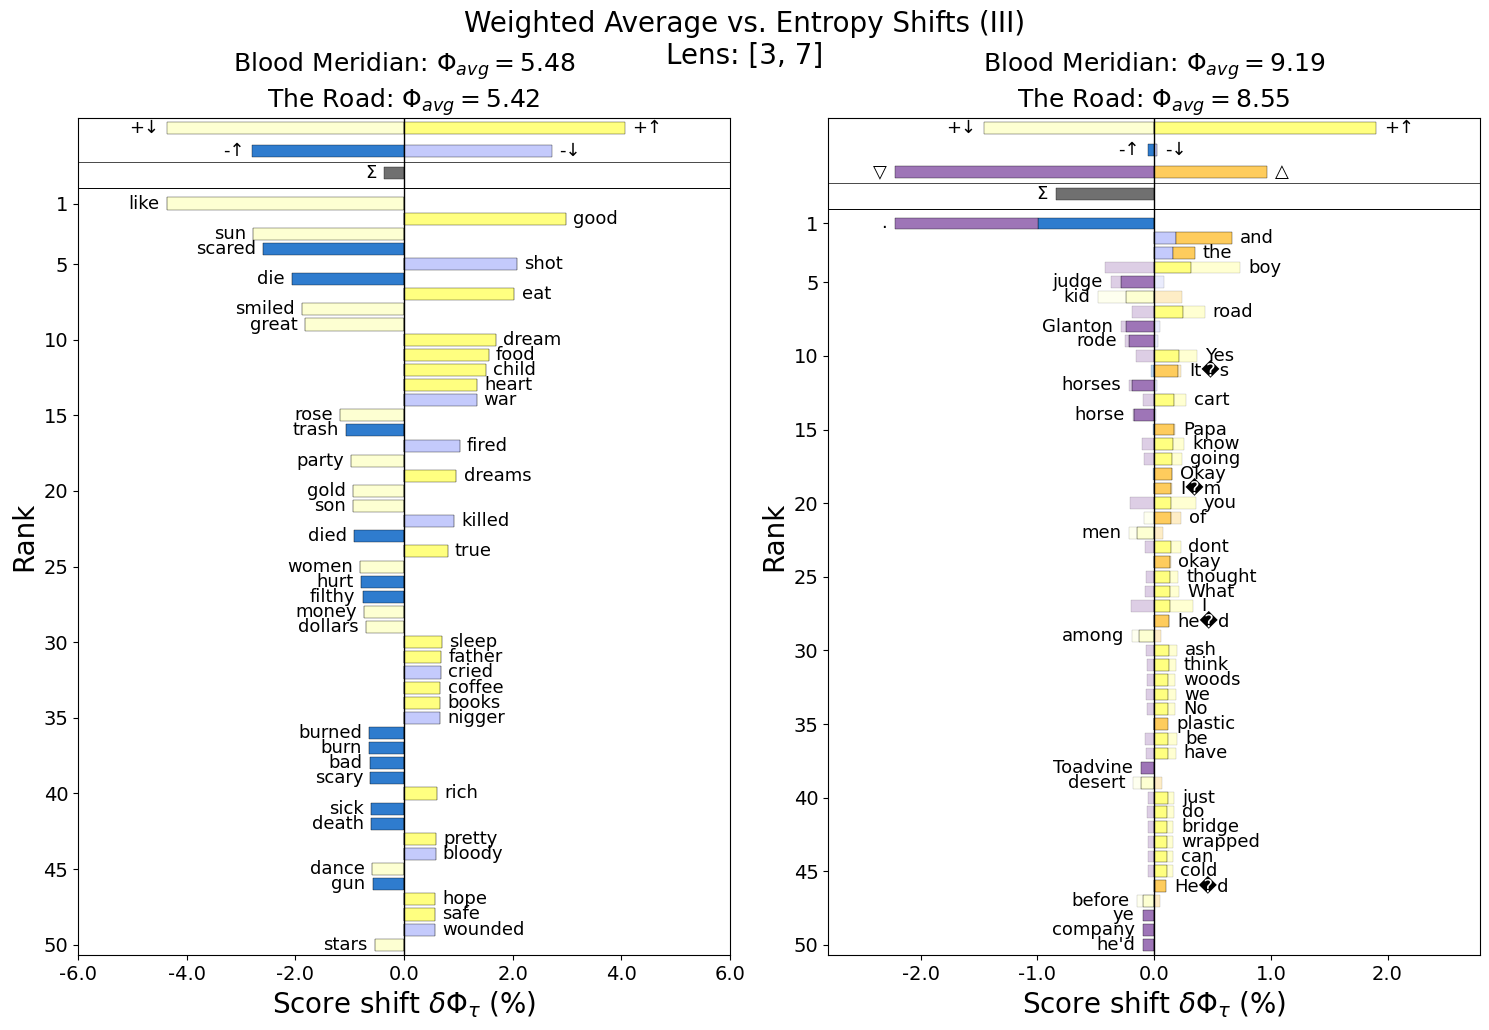
\includegraphics[width=\linewidth]{figures/21_1_e.png}
        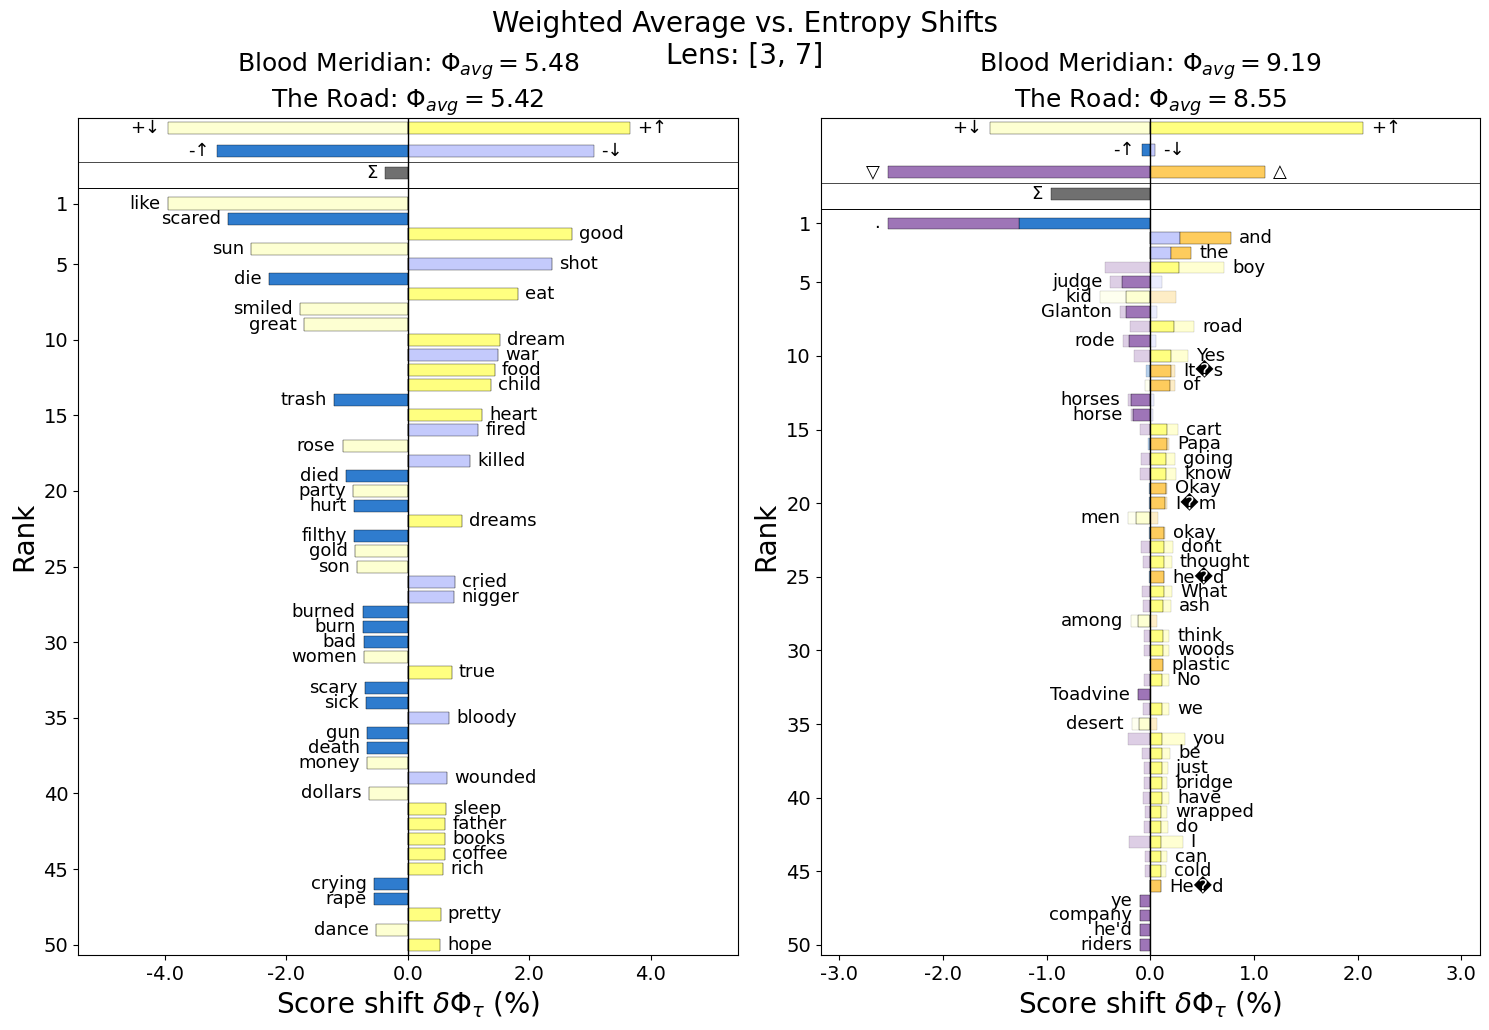
\includegraphics[width=\linewidth]{figures/21_1_a2.png}
    \end{center}
    
  \item
    % Compared to your first word shift, how interpretable is this one?

    Given that the average happiness of both texts is not significantly distant from 5, we do not see any startling changes.

    However, we do notice some of the more neutral words shifted lower (burned, burn, bad, women, etc.) which is to be expected if we are pretending that the happiness of these  words are not relative to the (con)text.

    I would say that they are both easily interpretable, understanding that the dictionary used to define the lexical happiness is neither exhaustive, nor is it necessarily appropriate to extend beyond the context of the relative comparisons that we have done thus far.

    In choosing the more appropriate reference value, we should err on the side of using the mean score of our reference text, as it is what we want to compare against.
    
  \end{enumerate}

   \solutionend

For additional viewing pleasure:

\begin{center}
    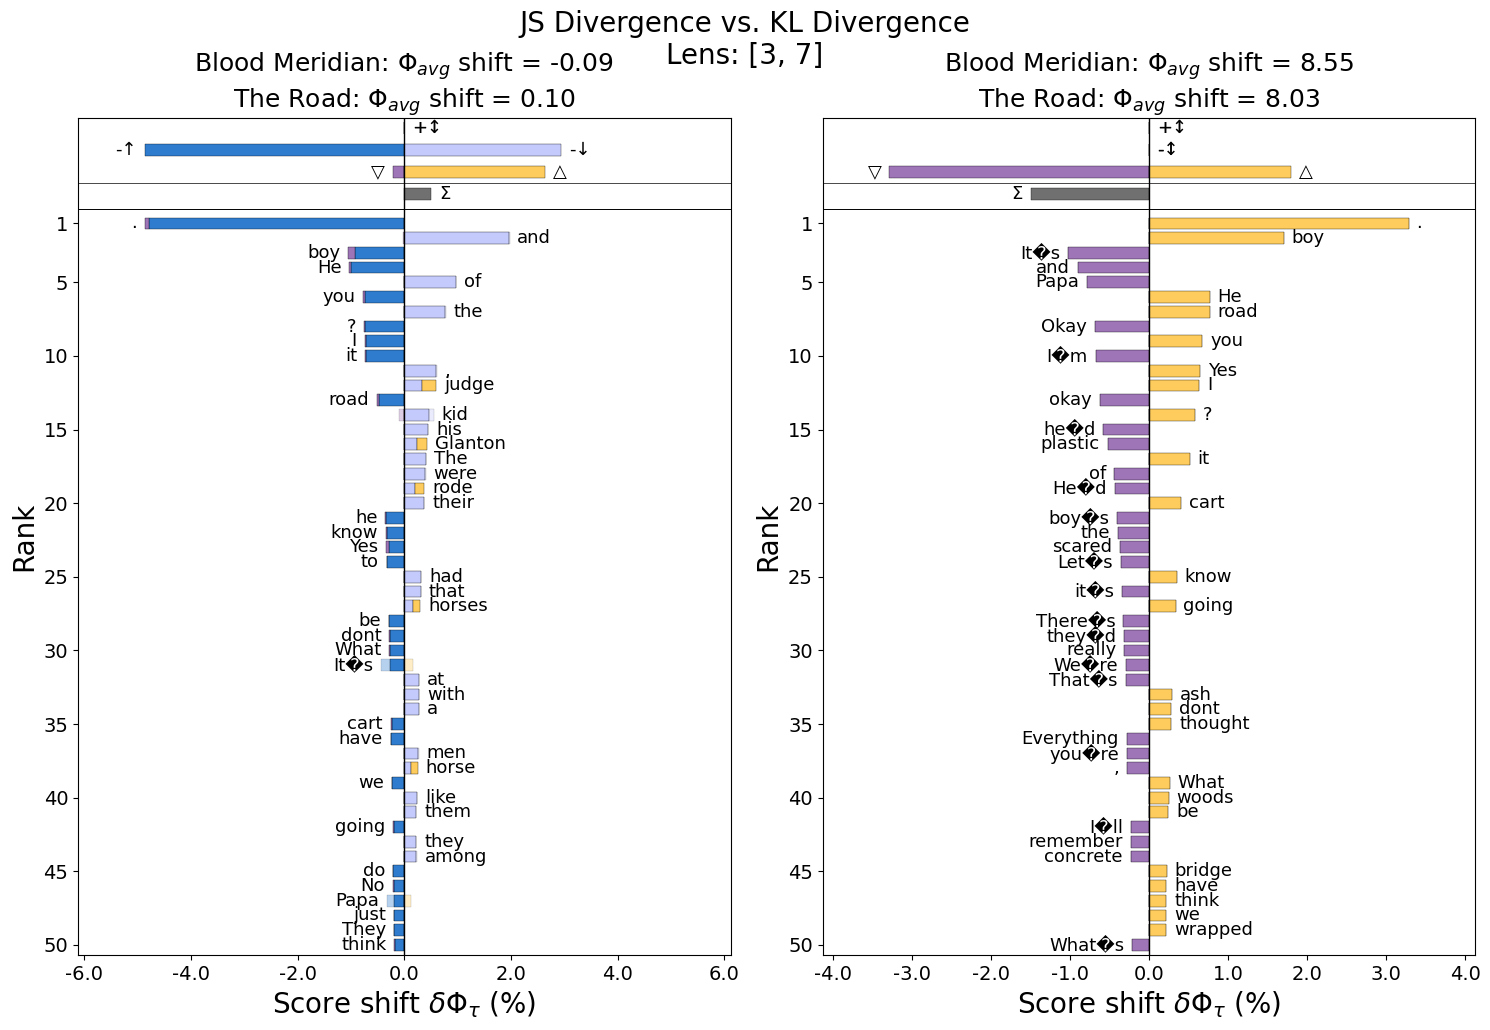
\includegraphics[width=\linewidth]{figures/jsd_kld.png}
\end{center}

\end{enumerate}

